%-------------------------------------------------------------------------------
\section{Prototype Design}
%-------------------------------------------------------------------------------
\label{sec:proto}

\begin{figure}[t!]
    \centering
    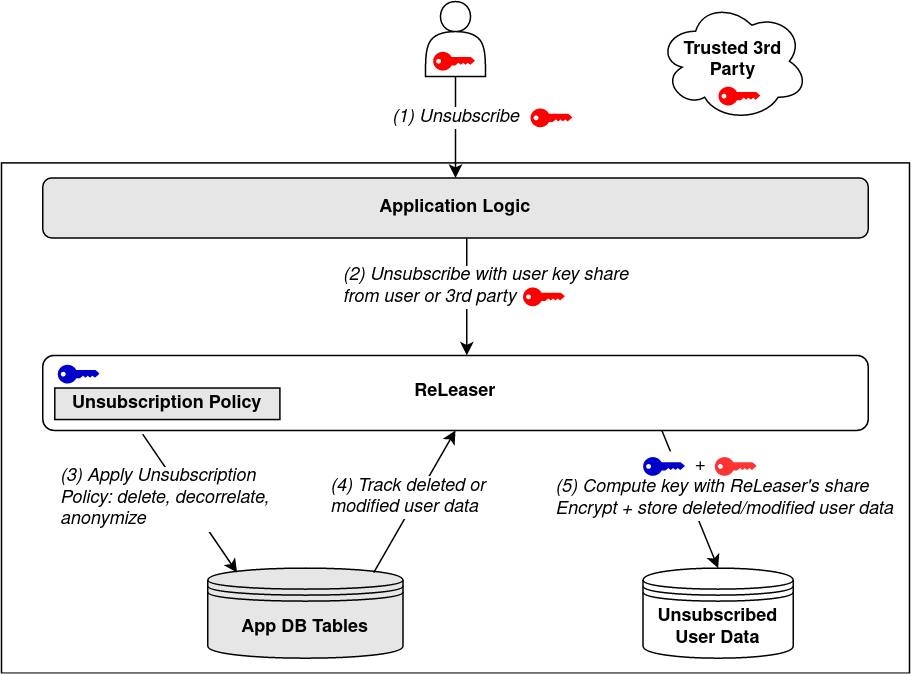
\includegraphics[width=0.5\textwidth]{img/releaser_arch}

    \caption{High-level \sys architecture. Developers specify grayed-out components.}
    \label{fig:arch}
\end{figure}

As shown in Figure~\ref{fig:arch}, \sys sits between the application logic and its database. \sys
models the application schema as an entity graph, and systematically applies the transformation
policies when invoked with the policy. 
If prompted, \sys will record the modifications performed during the transformation, and encrypts and
stores this log in an additional table. The encrypting key can be kept by the application for \eg content
moderation transformations, or in the case of user unsubscription, secret-shared~\cite{secretsharing}
among the user, \sys, and a trusted third party so that the user can retrieve a lost key without
trusting the application or \sys. To undo the transformation, \sys decrypts this log and reverses the
modifications, restoring the affected portion of the entity graph to its original state.

\sys consists of 5K LoC of Rust, and supports SQL queries as well as \texttt{TRANSFORM
[entity\_id]} and \texttt{REVERSE TRANSFORM [entity\_id]} queries.
We show that \sys performs reasonably (Section~\ref{sec:perf}), and we plan to support eventually
consistent, crash-recoverable transformations, sharding, and multicore parallelism.

%To amortize the cost of unsubscription and resubscription, \name preemptively creates, stores, and
%links ghost parent entities to child entities if an update creates an edge that may be decorrelated.
%\name builds in-memory materialized views on top of the underlying database, exposing ghost
%entities only if the true entity has been decorrelated, and real entities otherwise. Updates
%propagate to the materialized views when the underlying database is updated. \name answers
%application queries using these materialized views, hiding the complexity of ghost entity and
%decorrelation management.


